%%%%%%%%%%%%%%%%%%%%%%%%%%%%%%%%%%%%%%%%%%%%%%%%%%%%%%%%%%%%%%%%%%% VERBATIM CODE
\begin{verbatim}
        initial_values = []
\end{verbatim}
%%%%%%%%%%%%%%%%%%%%%%%%%%%%%%%%%%%%%%%%%%%%%%%%%%%%%%%%%%%%%%%%%%% ONE FIGURE
\begin{figure}[h]
  \centering
  \caption{Earth-Sun system}
  \subfloat[Euler.]{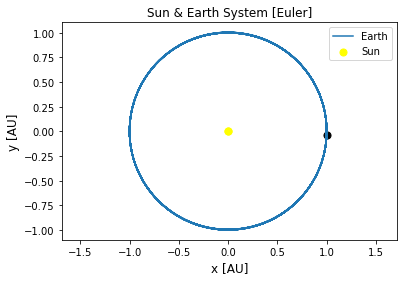
\includegraphics[width=0.5\textwidth]{euler.png}\label{fig:f1}}
  \hfill
  \subfloat[Verlet.]{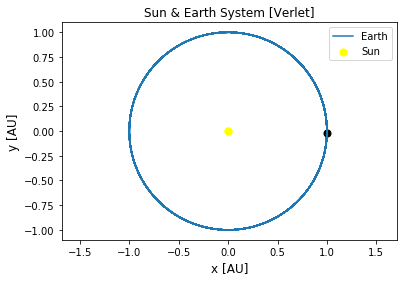
\includegraphics[width=0.5\textwidth]{verlet.png}\label{fig:f2}}
\end{figure}
%%%%%%%%%%%%%%%%%%%%%%%%%%%%%%%%%%%%%%%%%%%%%%%%%%%%%%%%%%%%%%%%%%% TWO FIGURE
\begin{figure}[h]
  \centering
   \caption{Stability plots, strongly zoomed.}
  \subfloat[Euler.]{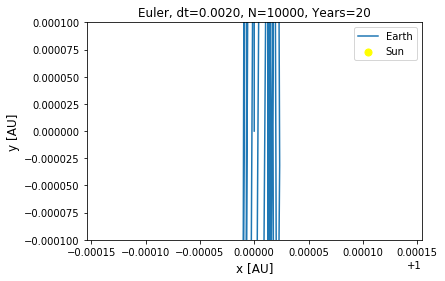
\includegraphics[width=0.5\textwidth]{euler_stab_dt002.png}\label{fig:f3}}
  \hfill
  \subfloat[Verlet.]{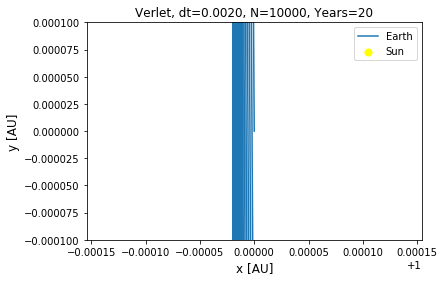
\includegraphics[width=0.5\textwidth]{verlet_stab_dt002.png}\label{fig:f4}}
\end{figure}
%%%%%%%%%%%%%%%%%%%%%%%%%%%%%%%%%%%%%%%%%%%%%%%%%%%%%%%%%%%%%%%%%%% TABLE
\begin{table}[h]
\caption{Conservation errors} % title of Table
\centering % used for centering table
\scalebox{0.8}{
\begin{tabular}{c c c c} % centered columns (4 columns)
\hline\hline %inserts double horizontal lines
Algorithm & Angular Momentum & Potential Energy & Kinetic Energy \\ [0.5ex] % inserts table
%heading
\hline % inserts single horizontal line
\\
Euler  & $1.80*10^{-19}$ & $8,83*10^{-11}$ & $8.94*10^{-11}$ \\ % inserting body of the table
Verlet & $3.66*10^{-19}$ & $4.12*10^{-17}$ & $3.89*10^{-17}$ \\[1ex]
\hline %inserts single line
\end{tabular}}
\label{table:nonlin} % is used to refer this table in the text
\end{table}
As seen in table [1], all quantities are conserved in terms of numerical expectation. Error calculation is made between initial values and final values.\\ Note that the Verlet algorithm yield less errors. [0.0002dt,100000n,20y]
\\
\begin{table}[!h]
\caption{Calculation time for 20 years [sec]} % title of Table
\centering % used for centering table
\scalebox{0.8}{
\begin{tabular}{c c c} % centered columns (4 columns)
\hline\hline %inserts double horizontal lines
dt & Euler & Verlet \\ [0.5ex] % inserts table
%heading
\hline % inserts single horizontal line
0.02 & 0.008 & 0.010 \\ % inserting body of the table
0.002 & 0.076 & 0.079 \\
0.0002 & 0.650 & 0.750 \\
0.00002 & 6.44 & 7.34 \\
0.000002 & 66.2 & 76.0 \\ [1ex] %[1ex] adds vertical space
\hline %inserts single line
\end{tabular}}
\label{table:nonlin} % is used to refer this table in the text
\end{table}